\section{Definieren des ersten neuronalen Netzes}
\label{chap:DefineNN}
Nachdem der Trainingsdatensatz definiert und in Ein- und Ausgabewerte aufgeteilt wurde, muss als Nächstes das \ac{NN} definiert werden, wie es Kapitel \ref{chap:Keras} beschriebt.
Dafür bietet die Keras-Bibliothek die Klasse \glqq Sequential\grqq{}, die genutzt werden kann, wenn Schichten sequentiell angeordnet werden sollen. Laut Chollet ist diese Art der 
Netzarchitektur die am häufigsten genutzte \cite[vgl. S.92]{DL_PY}. 

\begin{lstlisting}[language = python, caption={Erstellung eines sequentiellen Modells},captionpos=b, label = lst:ModellSeq, floatplacement=H]
    from keras.models import Sequential
    from keras.layers import Dense
    from keras.losses import CategoricalCrossentropy 

    model = Sequential()
    model.add(Dense(8, input_shape=(trainX.shape[1],), activation='relu'))
    model.add(Dense(16, activation='relu'))
    model.add(Dense(trainYStatus.shape[1], activation='softmax'))
\end{lstlisting}

Der Quellcode \ref{lst:ModellSeq} zeigt die benötigten Imports und wie ein Modell zur Vorhersage des Statuswerts definiert werden kann. Zuerst wird ein Objekt vom Typ Sequential erstellt. Diesem Objekt 
können dann die verschiedenen Schichten hinzugefügt werden. Dabei muss bestimmt werden, wie viele Schichten das Modell haben soll und wie viele Neuronen jede Schicht besitzen soll.
Als erste Schicht wird eine Dense-Layer als Eingabeschicht mit acht Neuronen definiert. Eine Dense-Layer ist eine fully-connected Schicht,
wie beispielsweise die Schichten in der Abbildung \ref{fig:NN_Modell}, und erwartet als Parameter mindestens die Anzahl an Neuronen. Optional können noch weitere Parameter angegeben werden.
Die Eingabeschicht benötigt als Besonderheit noch zusätzlich die Anzahl an Attributen, diese können dem Dataframe mit den Eingabewerten entnommen werden. Als Aktivierungsfunktion wird
die \ac{ReLU}-Funktion genutzt, die bereits in Kapitel \ref{chap:DL} vorgestellt wurde und auch die verbreitetste Aktivierungsfunktion beim \ac{DL} ist \cite[vgl. S.102]{DL_PY}. 
Als erste versteckte Schicht wird eine weitere Dense-Layer genutzt, hier mit 16 Neuronen. 
Die Anzahl an Neuronen und die Tiefe des Modells bestimmt die Komplexität des Modells. Ein zu komplexes Modell kann zu Überanpassung und ein zu simples Modell zu Unteranpassung führen.
Im Vorhinein ist es schwierig die benötigte Komplexität zu bestimmen, weshalb die Anzahl an Schichten und Neuronen, in Abhängigkeit zu dem Ergebnis des Modells, im Laufe der Erstellung noch geändert 
werden sollten. Als letzte Schicht und somit als Ausgabeschicht wird ebenfalls eine Dense-Layer verwendet. Die Anzahl an Neuronen in der Ausgabeschicht ist abhängig von der Anzahl an 
möglichen Ausprägungen des zu bestimmenden Wertes. Die ausgewählte Anwendungsregel wurde in der Vergangenheit mit \glqq closed\grqq{}, \glqq compliant\grqq{} und \glqq not applicable\grqq{} bewertet,
weshalb in diesem Fall die Ausgabeschicht drei Neuronen besitzen muss. Jedes Neuron stellt dabei eine mögliche Ausprägung dar. Anders als bei den vorherigen Schichten wurde bei dieser Schicht 
als Aktivierungsfunktion \glqq Softmax\grqq{} gewählt. Diese Aktivierungsfunktion weist jedem Neuron eine Wahrscheinlichkeit zwischen null und eins zu, wobei die Summe aller Wahrscheinlichkeiten 
eins ergibt \cite{KerasDoc}. Diese Eigenschaft der Funktion ist auch der Grund, weshalb für Status und Statement eigene Modelle erstellt werden müssen, da das Sequential-Modell nur eine Ausgabeschicht
erlaubt und es somit nicht möglich ist, mit dieser Funktion zwei Kategorien vorherzusagen. 

Die Auswahl der Aktivierungsfunktion der Ausgabeschicht ist abhängig von der Aufgabe des Modells. 
\glqq Softmax\grqq{} bietet sich zum Beispiel ideal als Möglichkeit zur Klassifikation an, wenn mehrere verschiedene Klassifizierungen vorhanden sind. Wenn nur zwei verschiedene Zustände möglich sind, 
also ein binäres Klassifikationsproblem vorliegt, würde sich als Aktivierungsfunktion eine Sigmoidfunktion anbieten, da diese beliebige Werte einen Ausgabebereich zwischen null und eins 
zuordnet \cite[vgl. S.100]{DL_PY}.

\begin{lstlisting}[language = python, caption={Zusammenfassung des Modells},captionpos=b, label = lst:ModellSummary, float, floatplacement=H]
    model.summary()
    ---------------------------------------
    Output:
    Model: "sequential"
    _______________________________________________________________
    Layer (type)                Output Shape              Param #   
    ===============================================================
    dense (Dense)               (None, 8)                 1424      
                                                                    
    dense_1 (Dense)             (None, 16)                144       
                                                                    
    dense_2 (Dense)             (None, 3)                 51        
                                                                    
    ===============================================================
    Total params: 1,619
    Trainable params: 1,619
    Non-trainable params: 0
    _______________________________________________________________
\end{lstlisting}
Eine Zusammenfassung wurde mit der summary()-Methode im Quellcode \ref{lst:ModellSummary} ausgegeben. 
Diese Zusammenfassung zeigt nochmal die verschiedenen Schichten, die Dimension der Ausgabe der Schichten sowie die Anzahl an Parametern in jeder Schicht an. 
Zu erkennen sind dort die drei hinzugefügten Dense-Layer. Die erste Dimension der Ausgabe ist \glqq None\grqq{}, da die Anzahl an Einträgen vorher nicht festgelegt wurde. 
Die zweite Dimension wird bestimmt durch die Anzahl an Neuronen in einer Schicht.\\

Je nach Anwendungsfall würden andere Schichten als die Dense-Layer infrage kommen. Stehen die Daten in einem sequentiellen Zusammenhang, beispielsweise eine Zeitreihe von Wetterdaten, dann würden
die sogenannten LSTM-Layer infrage kommen. LSTM steht für Long Short-Term-Memory(auf Deutsch: langes Kurzzeitgedächtnis) und diese Art von Schicht ist in der Lage Informationen mehrere Zeitschritte
lang zu erhalten \cite[vgl. S.260]{DL_PY}. Bei der Computer Vision werden häufig CNNs (Convolutional Neuronal Networks) genutzt. Ein CNN besteht dabei nicht aus Dense-Layern, wie in diesem 
Anwendungsfall, sondern aus Convolutional-Layern. Diese Schichten können zum Beispiel lokale Muster in Bildern erlernen und diese in neuen Bildern wiedererkennen, auch wenn sie nicht an derselben Stelle
sind \cite[vgl. S.164]{DL_PY}. Diese Schichten werden also in anderen Anwendungsfällen genutzt, für diesen Anwendungsfall eignen sich jedoch die Dense-Layer am besten.    \\

Bevor das Modell mit den Daten angelernt werden kann, müssen zunächst noch die Verlustfunktion und ein Optimierer ausgewählt werden. Da der Aufgabentyp eine Single-Label-Mehrfachklassifizierung 
ist, also eine Klassifizierung wo eine Klasse aus mehreren Klassen gewählt werden muss, wird als Verlustfunktion die kategorische Kreuzentropie genutzt. 
Eine Kreuzentropie misst die Differenz zwischen den vorhergesagten Wahrscheinlichkeiten und dem tatsächlichen Wert \cite[vgl. S.102]{DL_PY}.
Bei der kategorischen Kreuzentropie wird erwartet, dass die Ausgabewerte in der One-Hot-Codierung vorliegen. Sind die Ausgabewerte mit dem Label-Encoding codiert,
müsste als Verlustfunktion die \glqq Sparse Categorical Crossentropy\grqq{} genutzt werden \cite{KerasDoc}. Für andere Aufgabentypen werden andere 
Verlustfunktionen genutzt. Zum Beispiel bei einer Regression bietet sich der mittlere quadratische Fehler an oder bei der Binärklassifizierung die binäre Kreuzentropie \cite[vgl. S.155]{DL_PY}.
Während des Trainings wird das Modell versuchen das Ergebnis der kategorischen Kreuzentropie zu minimieren. 

Als Optimierer soll, laut Chollet, in den meisten Fällen der \glqq rmsprop\grqq{}-Optimierer mit der voreingestellten Lernrate verwendet werden können \cite[vgl. S.155]{DL_PY}. Ähnlich wie bei 
der Komplexität des Modells ist es schwierig vorher genau zu bestimmen, welcher Optimierer für die spezifische Anwendung die besten Ergebnisse liefert. Deshalb muss auch hier ausprobiert werden.
Zunächst wird sich an die Empfehlung von Chollet gehalten, es existieren jedoch auch weitere Optimierer, wie zum Beispiel \glqq Adam\grqq{} oder \glqq SGD\grqq{}, die berücksichtigt 
werden sollten \cite{KerasDoc}. 

Die Verlustfunktion sowie der Optimierer können nun, wie im Quellcode \ref*{lst:ModelCompile} gezeigt, ausgewählt werden. Diese werden der compile()-Methode als Parameter übergeben.
Zudem muss noch eine Kenngröße ausgewählt werden, die während des Anlernens überwacht wird. In diesem Fall wird dafür die \glqq categorical\_accuracy\grqq{} verwendet.
Diese Kenngröße gibt an, wie oft Vorhersagen den One-Hot codierten Ausgabewerten entsprechen.

\begin{lstlisting}[language = python, caption={Auswahl des Optimierers sowie der Verlustfunktion},captionpos=b, label = lst:ModelCompile, float, floatplacement=H]
    model.compile(optimizer='rmsprop',
        loss=CategoricalCrossentropy(),
        metrics=['categorical_accuracy'])
\end{lstlisting}

Nun ist das Modell fertig konfiguriert und kann auf den Trainingsdaten trainiert werden.

\subsection{Training des Modells}
\label{chap:TrainNN}

Zum Trainieren des Modells mit den vorher definierten und codierten Daten wird die fit()-Methode genutzt. Dieser Methode werden die Ein- und Ausgabewerte übergeben, mit dem das Modell trainiert werden soll.
Weitere Parameter sind:
\begin{description}[style=multiline,leftmargin=4cm,font=\bfseries, nolistsep]
    \item[batch\_size] Anzahl an Trainingsbeispielen, bevor die Gewichte des \ac{NN}~geupdatet werden \cite{KerasDoc}
    \item[epochs] Anzahl an Iterationen über den gesamten Trainingsdatensatz \cite{KerasDoc}
    \item[verbose] Bestimmt die Menge an Terminalausgaben \cite{KerasDoc}
    \item[validation\_split] Anteil des Trainingsdatensatzes, der zum Testen benutzt werden soll \cite{KerasDoc}
\end{description} 
Quellcode \ref*{lst:TrainModel} zeigt, wie hier die Parameter definiert wurden. In diesem ersten Trainingsansatz wurde als \glqq batch\_size\grqq{} zwei gewählt, was bedeutet, dass das Modell
nach jedem zweiten Trainingsbeispiel die Gewichte des Modells ändert. Da die ausgewählte Anwendungsregel lediglich 17-Mal bewertet wurde, muss die \glqq batch\_size\grqq{} dementsprechend niedrig gewählt
werden. Je niedriger die \glqq batch\_size\grqq{} ist, desto genauer kann das Modell die Trainingsdaten erlernen, was jedoch auch zu Overfitting führen kann. Zudem kann ein niedrigerer Wert 
die Laufzeit des Trainingsprozesses negativ beeinflussen, da das Modell häufiger geupdatet werden muss.

Die Anzahl an zu durchlaufenden Epochen wurde zunächst mit 50 gewählt. Hier muss ebenfalls im Nachhinein geprüft werden, wie viele Epochen benötigt werden. Eine höhere Anzahl an Epochen kann zu 
Overfitting führen, eine zu niedrige Anzahl zu Underfitting. Hier muss also mithilfe der Kenngröße geprüft werden, wie sich das Modell mit zunehmender/abnehmender Anzahl an Epochen verhält.

Für den Parameter \glqq verbose\grqq{} wurde der Wert zwei gewählt. Dieser sorgt dafür, dass die maximale Menge an Terminalausgaben ausgegeben wird. Ein Wert von eins würde nur einen 
Fortschrittsbalken ausgeben, ein Wert von null würde gar keine Ausgabe produzieren \cite{KerasDoc}.

Da ein Datensatz niemals mit den Trainingsdaten getestet werden sollte, muss eine Aufteilung in Testdaten erfolgen. Wie in Kapitel \ref*{chap:Trainingssplit} erwähnt, kann der Testsplit
während des Anlernens erfolgen. Dafür bietet Keras die Möglichkeit automatisch einen Teil der Trainingsdaten zum Testen zu benutzen.
In diesem Fall werden 25~\% des Datensatzes als Testdaten verwendet. Bei 17 Einträgen wären das 4,25 Einträge, die aber aufgerundet werden, also werden fünf Einträge 
nicht zum Trainieren benutzt, sondern werden fürs Testen zurückgehalten.

\begin{lstlisting}[language = python, caption={Trainieren des Modells},captionpos=b, label = lst:TrainModel, float, floatplacement=H]
    history = model.fit(trainX, trainYStatus,
                    batch_size=2,
                    epochs=50,
                    verbose=2,
                    validation_split=0.25)
\end{lstlisting}

\subsection{Testen des Modells}
\label{chap:TestNN}

Die Ausgabe des Trainingsprozesses kann dabei der Abbildung \ref*{fig:TrainModel} entnommen werden. Da der \glqq verbose\grqq{}-Wert auf zwei gesetzt wurde, wird für jede Epoche eine Ausgabe
generiert. Diese Ausgabe beinhaltet die benötigte Zeit für jede Epoche sowie den Wert der Verlustfunktion und der gewählten Kenngröße für die Trainings- und Testdaten.
\begin{figure}[H]
    \centering
    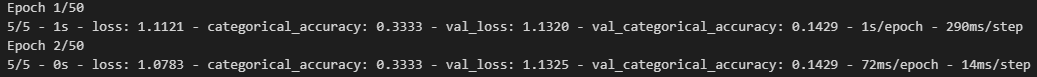
\includegraphics[width = \textwidth]{abbildungen/TrainAusgabe.png}
    \caption{Ausgabe des Trainingsprozesses}
    \label{fig:TrainModel}
\end{figure}
Der Wert der Verlustfunktion sowie die Genauigkeit können auch zusätzlich visualisiert werden, um den Verlauf darzustellen. Dazu wird das Objekt genutzt, welches bei Aufruf der 
fit()-Methode im Quellcode \ref*{lst:TrainModel} zurückgegeben und in der Variable \glqq history\grqq{} gespeichert wurde. Dieses Objekt beinhaltet 
den Wert der Verlustfunktion und die Genauigkeit für die Trainings- und Testdaten. Mithilfe der Matplotlib-Bibliothek können diese Werte dann in einem Liniendiagramm visualisiert werden,
der Quellcode \ref*{lst:PlotLoss} zeigt die benötigten Schritte für das Erstellen eines Liniendiagramms für die Verlustfunktion, die Genauigkeit kann jedoch äquivalent dazu 
dargestellt werden. Neben der Übergabe der Daten und der dazugehörigen Label können auch ein Titel und eine Achsenbeschriftung hinzugefügt werden, wie Zeile drei und vier des Quellcodes zeigen.
\begin{lstlisting}[language = python, caption={Trainieren des Modells},captionpos=b, label = lst:PlotLoss, float, floatplacement=H]
    plt.plot(history.history['loss'], label = 'Training loss')
    plt.plot(history.history['val_loss'], label = 'Validation loss')
    plt.title('Wert der Verlustfunktion')
    plt.xlabel('Epochen')
    plt.legend()
\end{lstlisting}
Abbildungen \ref*{fig:plotLoss} und \ref*{fig:plotAcc} zeigen die beiden erstellten Diagramme. Dort ist zu erkennen, dass mit zunehmender Anzahl an Epochen der Wert der Verlustfunktion abnimmt,
während die Genauigkeit zunimmt, was ein idealer Fall wäre. Die Werte sind jedoch mit Vorsicht zu betrachten, da sie nur ein Beispiel für ein Modell darstellen.
Da der Datensatz sehr klein ist, kann es sein, dass zufällig Testdaten ausgewählt wurden, die das Modell leichter erkennen konnte. Bei erneuter Ausführung könnten die 
Werte deshalb stark schwanken.

\begin{figure}[H]
    \centering
    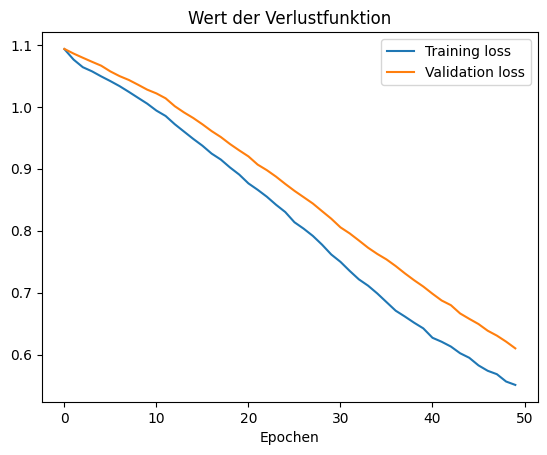
\includegraphics[width=.75\textwidth]{abbildungen/PlotLoss.png}
    \caption{Plot der Verlustfunktion}
    \label{fig:plotLoss}
\end{figure}
\begin{figure}[H]
    \centering
    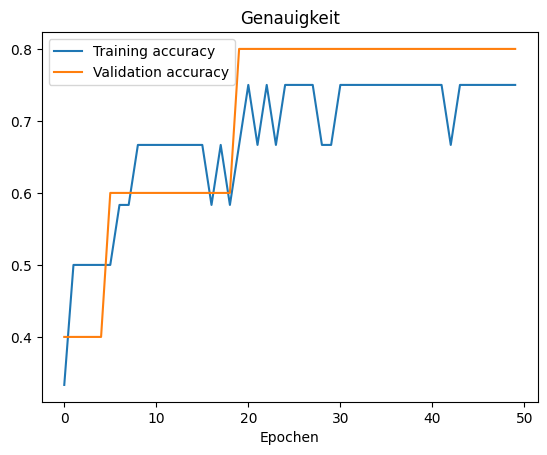
\includegraphics[width=.75\textwidth]{abbildungen/PlotAcc.png}
    \caption{Plot der Genauigkeit}
    \label{fig:plotAcc}
\end{figure}

\subsection{K-Cross-Validierung}
\label{chap:kCross}

Eine Möglichkeit zur besseren Beurteilung eines Modells wäre die k-cross-Validierung. Bei diesem Verfahren werden die Daten in k Teilmengen aufgeteilt
und k Modelle erstellt. Jedes Modell wird mit k-1 Teilmengen trainiert, die letzte Teilmenge wird zum Testen verwendet \cite[vgl. S.121f.]{DL_PY}. Abbildung \ref*{fig:kCross} zeigt
schematisch das Verfahren für k=3. Das endgültige Ergebnis ist definiert als der Durchschnitt der einzelnen Teilergebnisse der Modelle. 

\begin{figure}[H]
    \centering
    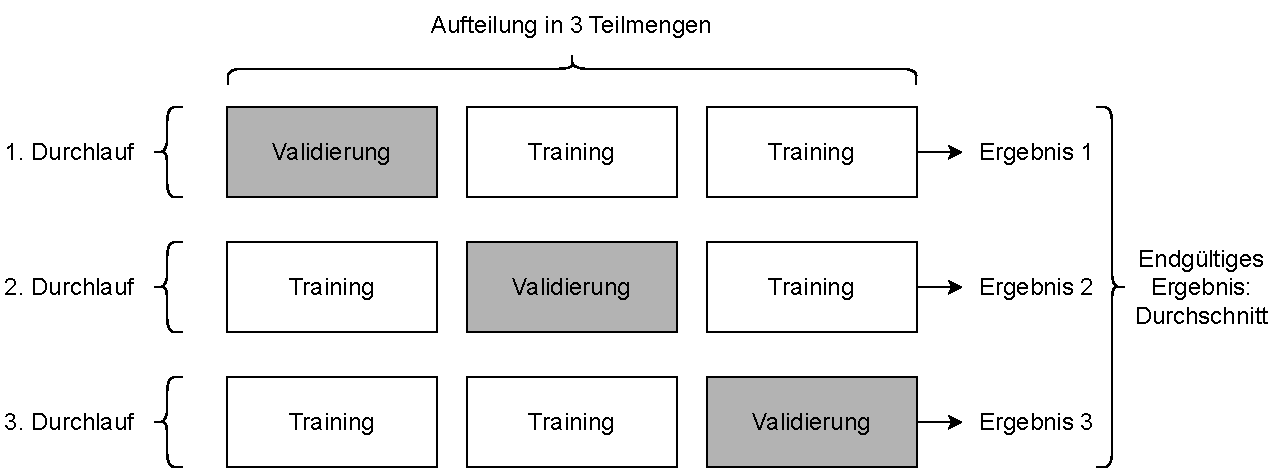
\includegraphics[width = \textwidth]{abbildungen/k_cross.pdf}
    \caption{k-cross-Validierung \cite[vgl. S.122]{DL_PY}}
    \label{fig:kCross}
\end{figure}

Um eine k-cross-Validierung durchzuführen, müssen nacheinander Modelle erstellt werden, die mit verschiedenen Teilmengen des Datensatzes trainiert und getestet werden.
Die dafür benötigten Schritte werden im Quellcode \ref*{lst:kCross} gezeigt.
Dafür wird als Erstes definiert, wie viele Modelle und Teilmengen genutzt werden sollen, hier wird sich für vier entschieden. 
Danach wird eine Schleife viermal durchlaufen und bei jeder Iteration wird der Trainings- und Testdatensatz neu definiert. Der Testdatensatz besteht dabei 
aus 25~\% des Datensatzes, in der ersten Iteration aus den ersten 25~\%, bei der zweiten die nächsten 25~\% und so weiter. Der Trainingsdatensatz beinhaltet die restlichen
Daten. Innerhalb der Schleife werden danach die Daten wieder in Ein- und Ausgabewerte aufgeteilt, dieses Mal müssen auch die Testdaten entsprechend aufgeteilt werden.
Danach kann wieder das Modell definiert und angelernt werden. Da der Testdatensatz nun selber definiert wurde, kann nicht mehr auf die automatische Aufteilung zurückgegriffen werden.
Jetzt müssen die Testdaten, aufgeteilt in Ein- und Ausgabewerte, der Methode übergeben werden. Zudem wurde hier die Anzahl an Epochen auf 250 erhöht, damit beobachtet werden kann,
wie das Modell sich bei steigender Anzahl an Epochen verhält. Das zurückgegebene Objekt der fit()-Methode wird genutzt, um die vier verschiedenen Werte jeweils in Listen speichern 
zu können, damit der Verlauf wieder visualisiert werden kann.
\begin{lstlisting}[language = python, caption={Aufteilung des Datensatzes in Teilmengen},captionpos=b, label = lst:kCross, float, floatplacement=H]
    num_epochs = 250
    k = 4
    for i in range(k):
        start = int(i/k * len(df_training))
        end = int((i/k + 0.25) * len(df_training))
        val_data = df_training.iloc[start:end] 
        train_data = df_training.drop(range(start,end))
        #...
        history = model.fit(trainX, trainYStatus,
                            batch_size=2,
                            epochs=num_epochs,
                            verbose=2,
                            validation_data=(valX, valYStatus))
        all_val_loss.append(history.history['val_loss'])
        all_loss.append(history.history['loss'])
        all_acc.append(history.history['categorical_accuracy'])
        all_val_acc.append(history.history['val_categorical_accuracy'])
\end{lstlisting}

Der Wert der Verlustfunktion sowie die Genauigkeit müssen noch gemittelt werden. Dafür wird, wie der Quellcode \ref*{lst:Durchschnitt} zeigt, der Durchschnitt 
der vier Kenngrößen pro Epoche gebildet. Mit den Werten können im nächsten Schritt wieder Diagramme zur Visualisierung erstellt werden.
\begin{lstlisting}[language = python, caption={Mitteln der Ergebnisse \cite{DL_PY}},captionpos=b, label = lst:Durchschnitt, floatplacement=H]
    avg_val_loss = [np.mean([x[i] for x in all_val_loss])
                    for i in range(num_epochs-1)]
    avg_loss     = [np.mean([x[i] for x in all_loss])
                        for i in range(num_epochs-1)]
    avg_acc      = [np.mean([x[i] for x in all_acc])
                        for i in range(num_epochs-1)]
    avg_val_acc  = [np.mean([x[i] for x in all_val_acc])
                        for i in range(num_epochs-1)]
\end{lstlisting}
Die Abbildungen \ref*{fig:kCrossLoss} und \ref*{fig:kCrossAcc} zeigen das Ergebnis der k-cross-Validierung. Bei der Verlustfunktion wird deutlich, dass
der Wert der Verlustfunktion auf den Testdaten bis ca. 80 Epochen leicht abnimmt, danach aber ansteigend, während der Wert der Verlustfunktion 
auf den Trainingsdaten abnimmt und gegen ca. 0,2 konvergiert. Das Ansteigen auf den Testdaten und Abnehmen auf den Trainingsdaten ist ein Zeichen dafür,
dass das Modell die Trainingsdaten auswendig lernt und die Generalisierungsfähigkeit des Modells darunter leidet und somit Overfitting auftritt.

Das Diagramm zur Genauigkeit zeigt, dass mehr Epochen nicht automatisch ein besseres Ergebnis liefern. Auf den Testdaten ändert sich die Genauigkeit 
ab der fünfzigsten Epoche nicht mehr wesentlich und stagniert ab Epoche 150. Im Vergleich zur Genauigkeit in der Abbildung \ref*{fig:plotAcc} 
ist der Durchschnitt der Genauigkeit von vier Modellen geringer. Daran kann erkannt werden, dass die Testdaten bei \ref*{fig:plotAcc} für das Modell günstig 
waren und das Modell auf diesen Daten gute Leistungen bringen konnte, was jedoch nicht so viel über die Leistung auf anderen Daten aussagt, da der Datensatz zu klein ist. 
Gerade in diesem Fall bietet sich die k-cross-Validierung sehr an und bietet wesentlich verlässlichere Kenngrößen als das Testen mit einem Modell auf einem 
Testdatensatz \cite[vgl. S.123]{DL_PY}.

\begin{figure}[H]
    \centering
    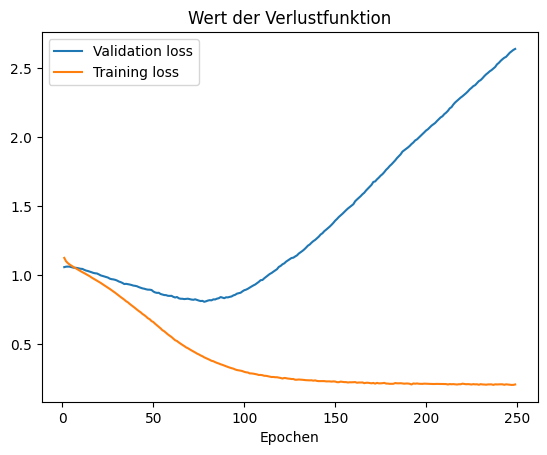
\includegraphics[width=.75\textwidth]{abbildungen/kCrossLoss.png}
    \caption{Verlustfunktion nach k-cross-Validierung}
    \label{fig:kCrossLoss}
\end{figure}
\begin{figure}[H]
    \centering
    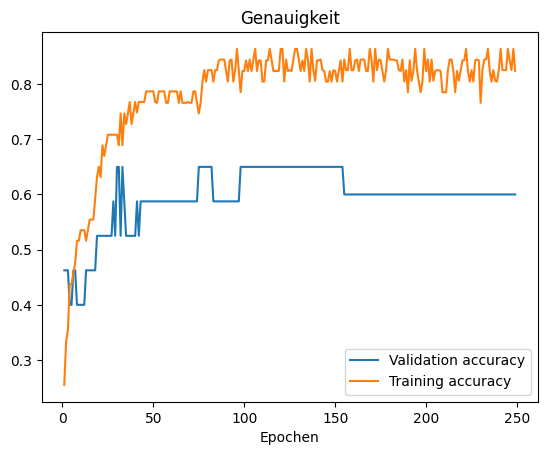
\includegraphics[width=.75\textwidth]{abbildungen/kCrossAcc.png}
    \caption{Genauigkeit nach k-cross-Validierung}
    \label{fig:kCrossAcc}
\end{figure}